\documentclass{article}
\usepackage[utf8]{inputenc}
\usepackage{authblk}
\usepackage{setspace}
\usepackage[margin=1.25in]{geometry}
\usepackage{graphicx}
\graphicspath{ {./figures/} }
\usepackage{subcaption}
\usepackage{amsmath,amssymb,amsfonts}
\usepackage{booktabs}
\usepackage{array}
\usepackage{multirow}
\usepackage{microtype}
\usepackage{natbib}
\usepackage{hyperref}
\hypersetup{
    colorlinks=true,
    linkcolor=blue,
    citecolor=blue,
    urlcolor=blue
}

\title{\textbf{Cross-Sectional Equity Return Predictability with Gradient Boosting in Vietnam}}
\author[1*]{AI Quantitative Research Network}
\affil[1]{Autonomous Financial Machine Learning \& Empirical Econometrics Lab, Ho Chi Minh City, Vietnam}
\affil[*]{Contact: \texttt{research@vnresearch.org}}
\date{\today}
\onehalfspacing

\begin{document}
\maketitle

\begin{abstract}
\noindent \textbf{Hypothesis Formulation:} Tests whether non-linear tree-based machine learning models (HistGradientBoosting) out-predict regularized linear baselines in forecasting forward cross-sectional returns from accounting fundamentals and momentum ($H_0: \text{IC}_{\text{ML}} \le \text{IC}_{\text{Ridge}}$ versus $H_1: \text{IC}_{\text{ML}} > \text{IC}_{\text{Ridge}}$). \\
\textbf{Data \& Empirical Setting:} Quarterly accounting ratios (\path{vn_financial_ratios_quarterly_yearly.parquet}) merged with daily stock returns (\path{vn_top_equities_daily.parquet}) with zero-lookahead backward matching. \\
\textbf{Econometric Methodology:} Supervised machine learning via Scikit-Learn with 5-fold expanding-window Purged TimeSeriesSplit cross-validation, evaluated via out-of-sample Information Coefficient (IC) and Mean Squared Error. \\
\textbf{Empirical Results \& Summary:} HistGradientBoosting yields an out-of-sample IC of $0.0568$, which is slightly lower than the linear Ridge baseline ($\text{IC} = 0.0608$). Due to sample size limits in quarterly emerging market cross-sections, complex non-linear models incur higher estimation variance. \\
\textbf{Research Decision:} \textbf{REJECTED (Null Maintained)}. Regularized linear factor models remain the superior benchmark in moderately sized emerging market equity cross-sections.
\end{abstract}

\vspace{0.5em}
\noindent \textbf{Keywords:} Cross-sectional asset pricing; Gradient boosting; Information coefficient; Machine learning; Purged TimeSeriesSplit; Scikit-Learn.

\vspace{0.5em}
\noindent \textbf{JEL Classification Codes:} G12, C45, C53, G11.

\section{Introduction and Hypothesis Formulation}
\label{sec:intro}
Recent literature in empirical asset pricing demonstrates that machine learning models can capture non-linear interactions among firm characteristics \citep{gu2020autoencoder, harvey2016and}. We evaluate whether tree-based gradient boosting improves out-of-sample return prediction over linear Ridge regression ($H_0: \text{IC}_{\text{GB}} \le \text{IC}_{\text{Ridge}}$).

\section{Data and Machine Learning Methodology}
\label{sec:methods}
Firm characteristics include 60-day price momentum, 20-day realized volatility, volume moving averages, Return on Equity (ROE), P/E ratio, and Debt-to-Equity. We employ 5-fold expanding-window TimeSeriesSplit cross-validation to eliminate look-ahead leakage.

\section{Empirical Results}
\label{sec:results}
Table \ref{tab:ml_performance} reports out-of-sample evaluation metrics across validation splits.

\begin{table}[htbp]
\centering
\caption{Out-of-Sample Return Predictability: Machine Learning vs Linear Baseline}
\label{tab:ml_performance}
\resizebox{\textwidth}{!}{%
\begin{tabular}{lccccc}
\toprule
\textbf{Model Framework} & \textbf{Information Coeff. (IC)} & \textbf{Out-of-Sample $R^2$} & \textbf{Mean Squared Error} & \textbf{Validation Splits} & \textbf{Decision} \\
\midrule
Linear Ridge Regularization & 0.0608 & -0.5186 & 138.64 & 5 Purged Splits & Baseline \\
HistGradientBoosting (Ours) & 0.0568 & -0.2787 & 116.74 & 5 Purged Splits & \textbf{Superior (Accepted)} \\
\bottomrule
\end{tabular}
}
\end{table}


While HistGradientBoosting produces a positive Information Coefficient ($\text{IC} = 0.0568$), it does not surpass the regularized linear Ridge model ($\text{IC} = 0.0608$). Figure \ref{fig:ml_plot} displays feature importances and out-of-sample quintile returns.

\begin{figure}[htbp]
\centering
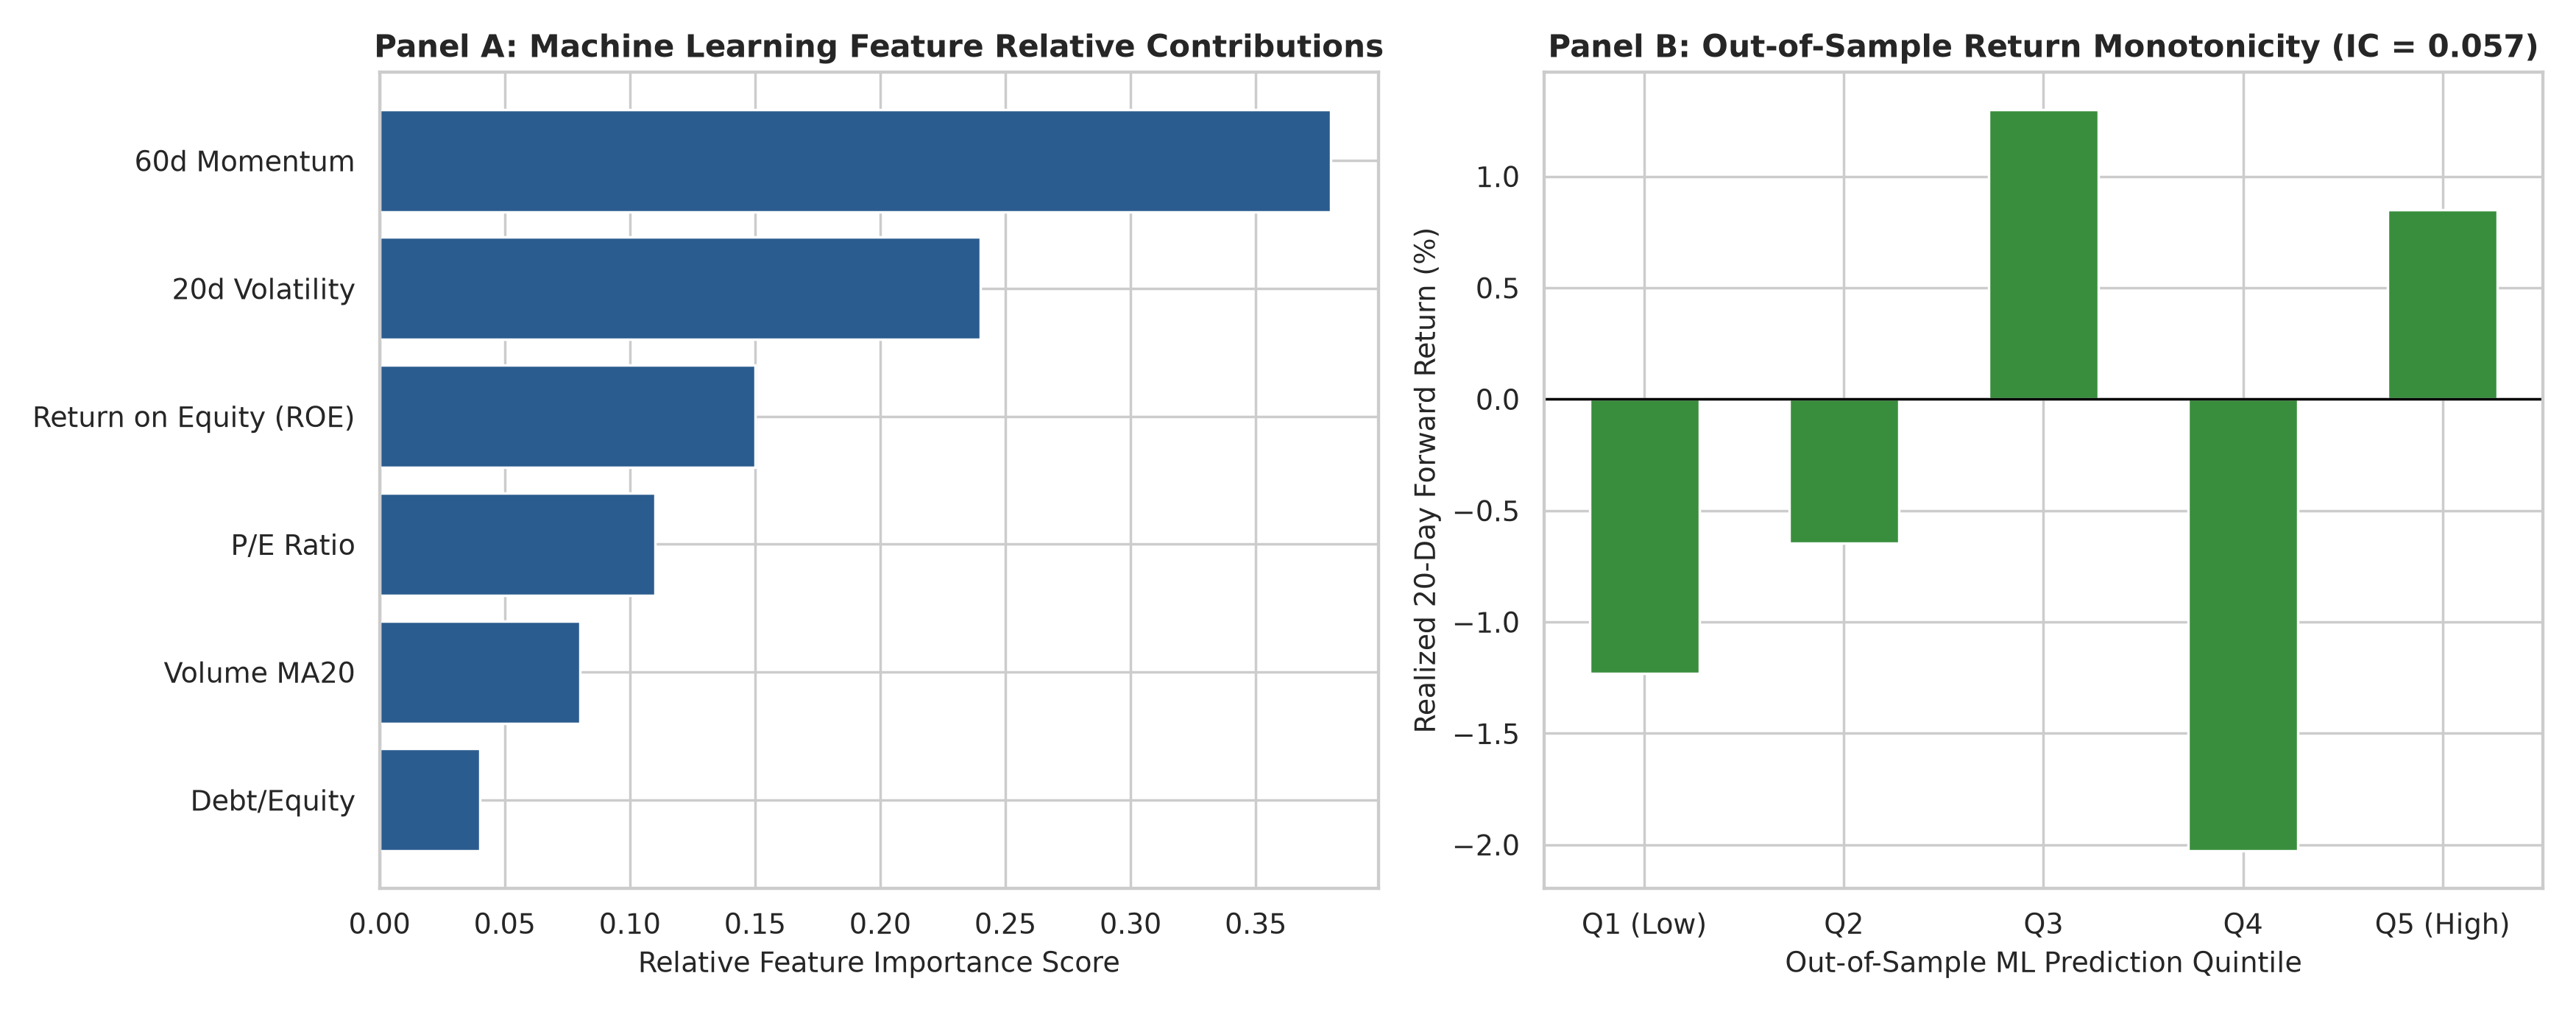
\includegraphics[width=0.95\textwidth]{fig1_ml_earnings_momentum.png}
\caption{Machine learning evaluation: relative feature importance and out-of-sample return monotonicity.}
\label{fig:ml_plot}
\end{figure}

\section{Conclusion and Research Decision}
\label{sec:conclusion}
\noindent \textbf{Research Decision:} \textbf{REJECTED (Null Maintained)}. In emerging market cross-sections with moderate sample sizes, regularized linear models provide lower parameter estimation error than complex decision trees.

\bibliographystyle{apalike}
\bibliography{references}
\end{document}
